
%% bare_jrnl.tex
%% V1.4b
%% 2015/08/26
%% by Michael Shell
%% see http://www.michaelshell.org/
%% for current contact information.
%%
%% This is a skeleton file demonstrating the use of IEEEtran.cls
%% (requires IEEEtran.cls version 1.8b or later) with an IEEE
%% journal paper.
%%
%% Support sites:
%% http://www.michaelshell.org/tex/ieeetran/
%% http://www.ctan.org/pkg/ieeetran
%% and
%% http://www.ieee.org/

%%*************************************************************************
%% Legal Notice:
%% This code is offered as-is without any warranty either expressed or
%% implied; without even the implied warranty of MERCHANTABILITY or
%% FITNESS FOR A PARTICULAR PURPOSE! 
%% User assumes all risk.
%% In no event shall the IEEE or any contributor to this code be liable for
%% any damages or losses, including, but not limited to, incidental,
%% consequential, or any other damages, resulting from the use or misuse
%% of any information contained here.
%%
%% All comments are the opinions of their respective authors and are not
%% necessarily endorsed by the IEEE.
%%
%% This work is distributed under the LaTeX Project Public License (LPPL)
%% ( http://www.latex-project.org/ ) version 1.3, and may be freely used,
%% distributed and modified. A copy of the LPPL, version 1.3, is included
%% in the base LaTeX documentation of all distributions of LaTeX released
%% 2003/12/01 or later.
%% Retain all contribution notices and credits.
%% ** Modified files should be clearly indicated as such, including  **
%% ** renaming them and changing author support contact information. **
%%*************************************************************************


% *** Authors should verify (and, if needed, correct) their LaTeX system  ***
% *** with the testflow diagnostic prior to trusting their LaTeX platform ***
% *** with production work. The IEEE's font choices and paper sizes can   ***
% *** trigger bugs that do not appear when using other class files.       ***                          ***
% The testflow support page is at:
% http://www.michaelshell.org/tex/testflow/



\documentclass[journal]{IEEEtran}
%
% If IEEEtran.cls has not been installed into the LaTeX system files,
% manually specify the path to it like:
% \documentclass[journal]{../sty/IEEEtran}





% Some very useful LaTeX packages include:
% (uncomment the ones you want to load)


% *** MISC UTILITY PACKAGES ***
%
%\usepackage{ifpdf}
% Heiko Oberdiek's ifpdf.sty is very useful if you need conditional
% compilation based on whether the output is pdf or dvi.
% usage:
% \ifpdf
%   % pdf code
% \else
%   % dvi code
% \fi
% The latest version of ifpdf.sty can be obtained from:
% http://www.ctan.org/pkg/ifpdf
% Also, note that IEEEtran.cls V1.7 and later provides a builtin
% \ifCLASSINFOpdf conditional that works the same way.
% When switching from latex to pdflatex and vice-versa, the compiler may
% have to be run twice to clear warning/error messages.






% *** CITATION PACKAGES ***
%
%\usepackage{cite}
% cite.sty was written by Donald Arseneau
% V1.6 and later of IEEEtran pre-defines the format of the cite.sty package
% \cite{} output to follow that of the IEEE. Loading the cite package will
% result in citation numbers being automatically sorted and properly
% "compressed/ranged". e.g., [1], [9], [2], [7], [5], [6] without using
% cite.sty will become [1], [2], [5]--[7], [9] using cite.sty. cite.sty's
% \cite will automatically add leading space, if needed. Use cite.sty's
% noadjust option (cite.sty V3.8 and later) if you want to turn this off
% such as if a citation ever needs to be enclosed in parenthesis.
% cite.sty is already installed on most LaTeX systems. Be sure and use
% version 5.0 (2009-03-20) and later if using hyperref.sty.
% The latest version can be obtained at:
% http://www.ctan.org/pkg/cite
% The documentation is contained in the cite.sty file itself.






% *** GRAPHICS RELATED PACKAGES ***
%
\ifCLASSINFOpdf
  % \usepackage[pdftex]{graphicx}
  % declare the path(s) where your graphic files are
  % \graphicspath{{../pdf/}{../jpeg/}}
  % and their extensions so you won't have to specify these with
  % every instance of \includegraphics
  % \DeclareGraphicsExtensions{.pdf,.jpeg,.png}
\else
  % or other class option (dvipsone, dvipdf, if not using dvips). graphicx
  % will default to the driver specified in the system graphics.cfg if no
  % driver is specified.
  % \usepackage[dvips]{graphicx}
  % declare the path(s) where your graphic files are
  % \graphicspath{{../eps/}}
  % and their extensions so you won't have to specify these with
  % every instance of \includegraphics
  % \DeclareGraphicsExtensions{.eps}
\fi
% graphicx was written by David Carlisle and Sebastian Rahtz. It is
% required if you want graphics, photos, etc. graphicx.sty is already
% installed on most LaTeX systems. The latest version and documentation
% can be obtained at: 
% http://www.ctan.org/pkg/graphicx
% Another good source of documentation is "Using Imported Graphics in
% LaTeX2e" by Keith Reckdahl which can be found at:
% http://www.ctan.org/pkg/epslatex
%
% latex, and pdflatex in dvi mode, support graphics in encapsulated
% postscript (.eps) format. pdflatex in pdf mode supports graphics
% in .pdf, .jpeg, .png and .mps (metapost) formats. Users should ensure
% that all non-photo figures use a vector format (.eps, .pdf, .mps) and
% not a bitmapped formats (.jpeg, .png). The IEEE frowns on bitmapped formats
% which can result in "jaggedy"/blurry rendering of lines and letters as
% well as large increases in file sizes.
%
% You can find documentation about the pdfTeX application at:
% http://www.tug.org/applications/pdftex





% *** MATH PACKAGES ***
%
%\usepackage{amsmath}
% A popular package from the American Mathematical Society that provides
% many useful and powerful commands for dealing with mathematics.
%
% Note that the amsmath package sets \interdisplaylinepenalty to 10000
% thus preventing page breaks from occurring within multiline equations. Use:
%\interdisplaylinepenalty=2500
% after loading amsmath to restore such page breaks as IEEEtran.cls normally
% does. amsmath.sty is already installed on most LaTeX systems. The latest
% version and documentation can be obtained at:
% http://www.ctan.org/pkg/amsmath





% *** SPECIALIZED LIST PACKAGES ***
%
%\usepackage{algorithmic}
% algorithmic.sty was written by Peter Williams and Rogerio Brito.
% This package provides an algorithmic environment fo describing algorithms.
% You can use the algorithmic environment in-text or within a figure
% environment to provide for a floating algorithm. Do NOT use the algorithm
% floating environment provided by algorithm.sty (by the same authors) or
% algorithm2e.sty (by Christophe Fiorio) as the IEEE does not use dedicated
% algorithm float types and packages that provide these will not provide
% correct IEEE style captions. The latest version and documentation of
% algorithmic.sty can be obtained at:
% http://www.ctan.org/pkg/algorithms
% Also of interest may be the (relatively newer and more customizable)
% algorithmicx.sty package by Szasz Janos:
% http://www.ctan.org/pkg/algorithmicx




% *** ALIGNMENT PACKAGES ***
%
%\usepackage{array}
% Frank Mittelbach's and David Carlisle's array.sty patches and improves
% the standard LaTeX2e array and tabular environments to provide better
% appearance and additional user controls. As the default LaTeX2e table
% generation code is lacking to the point of almost being broken with
% respect to the quality of the end results, all users are strongly
% advised to use an enhanced (at the very least that provided by array.sty)
% set of table tools. array.sty is already installed on most systems. The
% latest version and documentation can be obtained at:
% http://www.ctan.org/pkg/array


% IEEEtran contains the IEEEeqnarray family of commands that can be used to
% generate multiline equations as well as matrices, tables, etc., of high
% quality.




% *** SUBFIGURE PACKAGES ***
%\ifCLASSOPTIONcompsoc
%  \usepackage[caption=false,font=normalsize,labelfont=sf,textfont=sf]{subfig}
%\else
%  \usepackage[caption=false,font=footnotesize]{subfig}
%\fi
% subfig.sty, written by Steven Douglas Cochran, is the modern replacement
% for subfigure.sty, the latter of which is no longer maintained and is
% incompatible with some LaTeX packages including fixltx2e. However,
% subfig.sty requires and automatically loads Axel Sommerfeldt's caption.sty
% which will override IEEEtran.cls' handling of captions and this will result
% in non-IEEE style figure/table captions. To prevent this problem, be sure
% and invoke subfig.sty's "caption=false" package option (available since
% subfig.sty version 1.3, 2005/06/28) as this is will preserve IEEEtran.cls
% handling of captions.
% Note that the Computer Society format requires a larger sans serif font
% than the serif footnote size font used in traditional IEEE formatting
% and thus the need to invoke different subfig.sty package options depending
% on whether compsoc mode has been enabled.
%
% The latest version and documentation of subfig.sty can be obtained at:
% http://www.ctan.org/pkg/subfig




% *** FLOAT PACKAGES ***
%
%\usepackage{fixltx2e}
% fixltx2e, the successor to the earlier fix2col.sty, was written by
% Frank Mittelbach and David Carlisle. This package corrects a few problems
% in the LaTeX2e kernel, the most notable of which is that in current
% LaTeX2e releases, the ordering of single and double column floats is not
% guaranteed to be preserved. Thus, an unpatched LaTeX2e can allow a
% single column figure to be placed prior to an earlier double column
% figure.
% Be aware that LaTeX2e kernels dated 2015 and later have fixltx2e.sty's
% corrections already built into the system in which case a warning will
% be issued if an attempt is made to load fixltx2e.sty as it is no longer
% needed.
% The latest version and documentation can be found at:
% http://www.ctan.org/pkg/fixltx2e


%\usepackage{stfloats}
% stfloats.sty was written by Sigitas Tolusis. This package gives LaTeX2e
% the ability to do double column floats at the bottom of the page as well
% as the top. (e.g., "\begin{figure*}[!b]" is not normally possible in
% LaTeX2e). It also provides a command:
%\fnbelowfloat
% to enable the placement of footnotes below bottom floats (the standard
% LaTeX2e kernel puts them above bottom floats). This is an invasive package
% which rewrites many portions of the LaTeX2e float routines. It may not work
% with other packages that modify the LaTeX2e float routines. The latest
% version and documentation can be obtained at:
% http://www.ctan.org/pkg/stfloats
% Do not use the stfloats baselinefloat ability as the IEEE does not allow
% \baselineskip to stretch. Authors submitting work to the IEEE should note
% that the IEEE rarely uses double column equations and that authors should try
% to avoid such use. Do not be tempted to use the cuted.sty or midfloat.sty
% packages (also by Sigitas Tolusis) as the IEEE does not format its papers in
% such ways.
% Do not attempt to use stfloats with fixltx2e as they are incompatible.
% Instead, use Morten Hogholm'a dblfloatfix which combines the features
% of both fixltx2e and stfloats:
%
% \usepackage{dblfloatfix}
% The latest version can be found at:
% http://www.ctan.org/pkg/dblfloatfix




%\ifCLASSOPTIONcaptionsoff
%  \usepackage[nomarkers]{endfloat}
% \let\MYoriglatexcaption\caption
% \renewcommand{\caption}[2][\relax]{\MYoriglatexcaption[#2]{#2}}
%\fi
% endfloat.sty was written by James Darrell McCauley, Jeff Goldberg and 
% Axel Sommerfeldt. This package may be useful when used in conjunction with 
% IEEEtran.cls'  captionsoff option. Some IEEE journals/societies require that
% submissions have lists of figures/tables at the end of the paper and that
% figures/tables without any captions are placed on a page by themselves at
% the end of the document. If needed, the draftcls IEEEtran class option or
% \CLASSINPUTbaselinestretch interface can be used to increase the line
% spacing as well. Be sure and use the nomarkers option of endfloat to
% prevent endfloat from "marking" where the figures would have been placed
% in the text. The two hack lines of code above are a slight modification of
% that suggested by in the endfloat docs (section 8.4.1) to ensure that
% the full captions always appear in the list of figures/tables - even if
% the user used the short optional argument of \caption[]{}.
% IEEE papers do not typically make use of \caption[]'s optional argument,
% so this should not be an issue. A similar trick can be used to disable
% captions of packages such as subfig.sty that lack options to turn off
% the subcaptions:
% For subfig.sty:
% \let\MYorigsubfloat\subfloat
% \renewcommand{\subfloat}[2][\relax]{\MYorigsubfloat[]{#2}}
% However, the above trick will not work if both optional arguments of
% the \subfloat command are used. Furthermore, there needs to be a
% description of each subfigure *somewhere* and endfloat does not add
% subfigure captions to its list of figures. Thus, the best approach is to
% avoid the use of subfigure captions (many IEEE journals avoid them anyway)
% and instead reference/explain all the subfigures within the main caption.
% The latest version of endfloat.sty and its documentation can obtained at:
% http://www.ctan.org/pkg/endfloat
%
% The IEEEtran \ifCLASSOPTIONcaptionsoff conditional can also be used
% later in the document, say, to conditionally put the References on a 
% page by themselves.




% *** PDF, URL AND HYPERLINK PACKAGES ***
%
%\usepackage{url}
% url.sty was written by Donald Arseneau. It provides better support for
% handling and breaking URLs. url.sty is already installed on most LaTeX
% systems. The latest version and documentation can be obtained at:
% http://www.ctan.org/pkg/url
% Basically, \url{my_url_here}.




% *** Do not adjust lengths that control margins, column widths, etc. ***
% *** Do not use packages that alter fonts (such as pslatex).         ***
% There should be no need to do such things with IEEEtran.cls V1.6 and later.
% (Unless specifically asked to do so by the journal or conference you plan
% to submit to, of course. )


% correct bad hyphenation here
\hyphenation{op-tical net-works semi-conduc-tor}


% use for special paper notices
%\IEEEspecialpapernotice{(Invited Paper)}

\usepackage{amsmath}
\usepackage{graphicx}
\usepackage{booktabs} % For formal tables
%\usepackage{algorithm}
%\usepackage{algorithmic}
%\usepackage[]{algorithm2e}
%\usepackage{algpseudocode}
\usepackage{algorithm}
\usepackage{algorithmicx}
\usepackage[noend]{algpseudocode}
%\usepackage[belowskip=-10pt,aboveskip=-2pt]{caption}

\usepackage{todonotes,soul}
\usepackage{xcolor}


\newcommand{\highlight}[1]{\textcolor{red}{#1}}
\newcommand{\caj}[1]{\todo[inline,linecolor=organge,backgroundcolor=orange!25,bordercolor=orange]{AJ: #1}}
\newcommand{\cajb}[1]{\todo[linecolor=orange,backgroundcolor=orange!25,bordercolor=orange]{AJ: #1}}

\newcommand{\cmw}[1]{\todo[inline,linecolor=green,backgroundcolor=green!25,bordercolor=green]{MW: #1}}
\newcommand{\cmwb}[1]{\todo[linecolor=green,backgroundcolor=green!25,bordercolor=green]{MW: #1}}


\begin{document}
%
% paper title
% Titles are generally capitalized except for words such as a, an, and, as,
% at, but, by, for, in, nor, of, on, or, the, to and up, which are usually
% not capitalized unless they are the first or last word of the title.
% Linebreaks \\ can be used within to get better formatting as desired.
% Do not put math or special symbols in the title.
\title{Bare Demo of IEEEtran.cls\\ for IEEE Journals}
%
%
% author names and IEEE memberships
% note positions of commas and nonbreaking spaces ( ~ ) LaTeX will not break
% a structure at a ~ so this keeps an author's name from being broken across
% two lines.
% use \thanks{} to gain access to the first footnote area
% a separate \thanks must be used for each paragraph as LaTeX2e's \thanks
% was not built to handle multiple paragraphs
%

\author{Matthias~Wess,
        Sai~D.P.,~\IEEEmembership{Fellow,~OSA,}
        and~Jane~Doe,~\IEEEmembership{Life~Fellow,~IEEE}% <-this % stops a space
\thanks{M. Shell was with the Department
of Electrical and Computer Engineering, Georgia Institute of Technology, Atlanta,
GA, 30332 USA e-mail: (see http://www.michaelshell.org/contact.html).}% <-this % stops a space
\thanks{J. Doe and J. Doe are with Anonymous University.}% <-this % stops a space
\thanks{Manuscript received April 19, 2005; revised August 26, 2015.}}

% note the % following the last \IEEEmembership and also \thanks - 
% these prevent an unwanted space from occurring between the last author name
% and the end of the author line. i.e., if you had this:
% 
% \author{....lastname \thanks{...} \thanks{...} }
%                     ^------------^------------^----Do not want these spaces!
%
% a space would be appended to the last name and could cause every name on that
% line to be shifted left slightly. This is one of those "LaTeX things". For
% instance, "\textbf{A} \textbf{B}" will typeset as "A B" not "AB". To get
% "AB" then you have to do: "\textbf{A}\textbf{B}"
% \thanks is no different in this regard, so shield the last } of each \thanks
% that ends a line with a % and do not let a space in before the next \thanks.
% Spaces after \IEEEmembership other than the last one are OK (and needed) as
% you are supposed to have spaces between the names. For what it is worth,
% this is a minor point as most people would not even notice if the said evil
% space somehow managed to creep in.



% The paper headers
\markboth{IEEE TRANSACTIONS ON COMPUTER-AIDED DESIGN OF INTEGRATED CIRCUITS AND SYSTEMS}%
{Shell \MakeLowercase{\textit{et al.}}: Bare Demo of IEEEtran.cls for IEEE Journals}
% The only time the second header will appear is for the odd numbered pages
% after the title page when using the twoside option.
% 
% *** Note that you probably will NOT want to include the author's ***
% *** name in the headers of peer review papers.                   ***
% You can use \ifCLASSOPTIONpeerreview for conditional compilation here if
% you desire.




% If you want to put a publisher's ID mark on the page you can do it like
% this:
%\IEEEpubid{0000--0000/00\$00.00~\copyright~2015 IEEE}
% Remember, if you use this you must call \IEEEpubidadjcol in the second
% column for its text to clear the IEEEpubid mark.






% make the title area
\maketitle

% As a general rule, do not put math, special symbols or citations
% in the abstract or keywords.


%%%%%%%%%%%%%%%%%%%%%%%%%%%%%%%%%%%%%%%%%%%%%%%%%%%%%%%%%%%%%%%%%%%%%%%%%%%%%%%%
\begin{abstract}
Deployment of Deep Neural Networks (DNNs) on hardware platforms 
is often constrained by limited on-chip memory and computational power. 
The proposed weight quantization offers the possibility of optimizing weight memory alongside transforming the weights to hardware friendly data-types. 
We apply \emph{Dynamic Fixed Point} and \emph{Power-of-two quantization} in conjunction with \emph{Layer-wise Precision Scaling} to minimize the weight memory. To alleviate accuracy degradation due to precision scaling, we employ 
quantization-aware fine-tuning.
For fine-tuning, \emph{quantization-regularization} and \emph{weighted quantization-regularization} are introduced 
to force the trained quantization by adding the distance of the weights to the desired quantization levels as a regularization term to the loss-function. While Dynamic Fixed Point quantization performs better when allowing different bit-widths for each layer, Power-of-two quantization in combination with retraining allows higher compression rates for equal bit-width quantization.
The techniques are verified on an All-Convolutional Network. With a maximum accuracy degradation of 0.10 percentage points, for Dynamic Fixed Point with Layer-wise Precision Scaling we achieve compression ratios of $7.34$ for CIFAR-10, $4.7$ for CIFAR-100 and $9.33$ for SVHN dataset.
%\todo[inline]{Can we mention as On average, the proposed technique achieves xyz$\times$ compression for dynamic fixed point and power-of-two quantization with a maximum accuracy degradation of 1\% on tested datasets.}
\end{abstract}

%As external memory access is compared to computations the most expensive operation by measures of power-consumption, many works focus on model compression and efficient buffering to reduce the transferred data.



% Note that keywords are not normally used for peerreview papers.
\begin{IEEEkeywords}
IEEE, IEEEtran, journal, \LaTeX, paper, template.
\end{IEEEkeywords}






% For peer review papers, you can put extra information on the cover
% page as needed:
% \ifCLASSOPTIONpeerreview
% \begin{center} \bfseries EDICS Category: 3-BBND \end{center}
% \fi
%
% For peerreview papers, this IEEEtran command inserts a page break and
% creates the second title. It will be ignored for other modes.
\IEEEpeerreviewmaketitle




%%%%%%%%%%%%%%%%%%%%%%%%%%%%%%%%%%%%%%%%%%%%%%%%%%%%%%%%%%%%%%%%%%%%%%%%%%%%%%%%
\section{Introduction}
\label{sec:intro}
\IEEEPARstart{S}{tarting} with AlexNet \cite{Krizhevsky2012} Deep Convolutional Neural Networks (DCNN) have been gaining attention by delivering impressive results on challenging problems, such as object recognition on ImageNet dataset \cite{Deng2009} or facial recognition \cite{Taigman2014}. 
The adaptation of such DCNNs and deep neural networks (DNNs) in various 
applications including autonomous driving, medical diagnosis \cite{Rajpurkar2017} and machine translation \cite{Zhang2015a} led to an 
ever increasing amounts of data to process under high performance requirements. 
%speeds a large field of applications as opened up, including .

Most of these applications can be described as supervised learning tasks, 
split into training phase and inference. In the training phase, 
the algorithm is optimized to solve a certain task for the training data. The 
architecture of a DCNN or DNN is defined by the number of layers and their 
functionality (e.g. Convolutional, Fully Connected, Pool, Batch-Normalization) 
and the layer-specific parameters which define the dimensions and behavior of the 
layer in forward and backward-propagation. To train the defined architecture on a 
given training data, the labeled data is fed through the network and 
in back-propagation, the layer-specific weights are adjusted to decrease the error between the output and original label. For inference, DNN employs the model derived during training phase on the test or unknown data. 
The ability to correctly process the new data based on training data
is called generalization ability.

Despite state-of-the-art DNNs taking one or several high-end GPUs 
and up to several days to train, inference can be performed on 
a broad spectrum of platforms including CPUs, GPUs, FPGAs, and ASICs. 
With the increasing size of DNNs (e.g. ResNet \cite{He2016} up to 152 layers), even the complexity of inference is also exacerbating 
due to more critical requirements and constraints such as limited power consumption, high throughput or hard real-time processing. 
There are several challenges that hinder the efficient deployment and 
inference of the State-of-the-art Deep Neural Networks (DNN) on embedded 
resource constrained platforms. The two biggest challenges are the 
large size of the networks and the total number of necessary operations in feed-forward computation, since a hardware accelerator design can be bound either by the limit of parallel operations, or by the memory interface transmission rate \cite{Zhang2015}. As a consequence, model compression and increasing the efficiency of computations, are two legitimate ways to reach hardware requirements.

Recent works \cite{Han2015,Zhou2017a} have proven the robustness of DNNs 
to compression of weights and simplification of activation functions with 
high number of parameters and the resulting redundancy \cite{Han2015, Chen2017, Lin2015a, Courbariaux2014}. This enables several techniques including weight sharing \cite{Han2015, Dong2017}, pruning \cite{Han2015a} and Huffman Encoding \cite{Han2015} to reduce external memory access. Pruning not only reduces the memory footprint of a DNN model, but also allows skipping of multiplications with 0, thus reducing the amount of total multiplications \cite{Yang2017, Yu2017}. To reduce also power consumption within operations, the model parameters have to be quantized in specific formats a dedicated hardware can make use of.
%\cmw{\textcolor{red}{What's the problem or short coming? In other terms why should we something if these solutions solve everything} The sentence was a bit confusing. Pruning is solved but the problem is quantization for efficient hardware inference}
Dynamic fixed point \cite{Courbariaux2014, Gysel2016a} and power of two quantization \cite{Zhou2017a} are two hardware friendly formats that enable performing multiplications either as low-precision multiplications or simple shift operations. %Furthermore recent research suggests that hardware porting techniques such as training the network with ternary \cite{Alemdar2016} or binary weights \cite{Courbariaux2015, Kim2016, Tang2017, Hou2016} networks is efficient.
%In addition to solely quantizing weights, also layer output maps can be quantized, thus reducing bit-width of not just one factor of each multiplication, but of both factors\cite{Gysel2018}. Due to evolving training strategies, networks employing binary activations and binary weights are reaching increasing accuracies for most tasks \cite{Hubara2016b, Rastegari2016}. \textcolor{red}{Are we using binary even in DFP?} \cmw{no, lowest possbile with DFP is 2 bit which means ternary. DFP has always one sign bit therefore binary would be +0 and -0}

There are several approaches on how to best prepare a DNN for inference with 
low precision data types. On one side when employing the state-of-the-art DNNs 
it is desirable to directly make use of pre-trained models without architectural
adjustments. \cite{Lin2015a} and \cite{Zhou2017} propose methods for layer-wise 
bit-width optimization without retraining but not for bit-width optimization 
followed by retraining. Furthermore, to fully leverage optimized hardware 
accelerators for efficient inference (e.g.\cite{han2016eie}) it can be desirable 
to force certain quantization \cite{Zhou2017a}, compression or pruning schemes 
\cite{Yang2017} in an additional fine-tuning step. \cite{Zhou2017a} proposes 
incremental weight quantization while incorporating a Power-of-two datatype and 
achieve almost lossless quantization for several DNNs. Other works such as 
\cite{Gysel2016, Hubara2016} employ stochastic quantization methods to during 
training. In stochastic training the algorithm stores a floating point value and 
the quantized value at the same time and for each feed forward computation the 
quantized weights are newly computed on a stochastic basis.

%\textcolor{red}{Mention a very high-level overview of the paper in a single paragraph, bit more details than that in the contributions.}

%\subsection{Main contributions}
\vspace{2ex}
This paper makes the following contributions:
\begin{itemize}
%quantization during training
%any quantization scheme
%could be also applied per filter, on batchnorm
\item We propose weighted quantization-regularization (WQR), a method for trained low precision quantization of weights in Neural Networks to any given quantization scheme.

\item We combine Layer-wise Precision Scaling \cite{Zhou2017} with weighted quantization-regularization to reduce the loss in classification performance while increasing the compression rate.

\item We analyze the benefits of Power-of-2 (Po2) and Dynamic Fixed Point (DFP) based quantization in our setting and in combination with weighted quantization-regularization and layer-wise bit-width optimization.
\end{itemize}

Aiming at highly efficient implementation in FPGAs, we perform evaluation 
for quantization-regularization for dynamic fixed point \cite{Hubara2016} and 
power of two quantization \cite{Zhou2017a} schemes on CNNs. We apply the proposed 
algorithm on SVHN CIFAR-10 and CIFAR-100 dataset for two different quantization schemes and show that weighted quantization-regularization decreases loss in classification performance in comparison to direct weight quantization for All-Convolutional Network on CIFAR-10 from 1.5\% to 0\%. The results suggest that the proposed algorithm reduces accuracy loss due to quantization of CNNs.



%\subsection{Organization of the paper}

%In this paper we first explain in a motivational case study





%%%%%%%%%%%%%%%%%%%%%%%%%%%%%%%%%%%%%%%%%%%%%%%%%%%%%%%%%%%%%%%%%%%%%%%%%%%%%%%%
\begin{figure}[ht!]
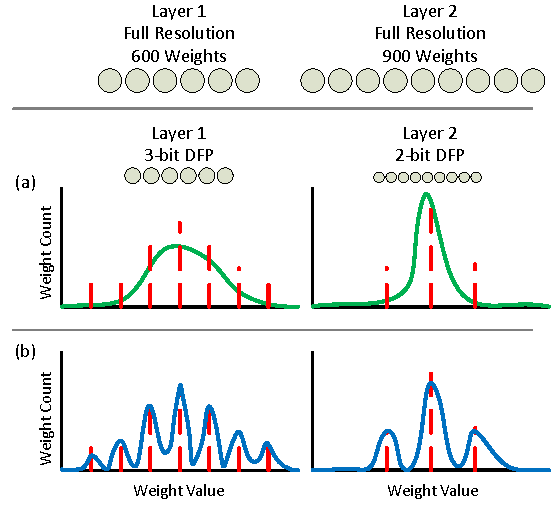
\includegraphics[width=\columnwidth]{img/intro2.pdf}
\caption{An example Network with two layers demonstrating (a) Layer-wise Precision Scaling (b) Retraining with Quantization-regularization. Starting with two layer network at first the bit-widths of both layers are adjusted by defining a lower precision format with the quantization levels marked as dotted lines in the histogram charts (a). To reduce the quantization error, retraining with additional regularization, decreasing the average distance of the weights to the quantization levels, is performed (b).}\label{fig:intro}
\end{figure}


\section{Motivational Case Study}
%The method proposed in this paper attacks the two biggest challenges for efficient DNN inference on resources restricted devices (\ref{sec:intro}). 
Figure \ref{fig:intro} explains with a simple example the two main parts of the paper. Assuming a two-layer neural network with two layers with 600 and 900 weights respectively, we want to achieve model compression by reducing the number of bits stored per weight and specific quantization of the weights to enhance the computational energy efficiency. 

First note, that layer 2 has a stronger impact on the size of the weight memory, as it contains more weights. Thus, it is beneficial in terms of memory footprint to reduce the bit-width of its weights more than those of layer 1. 
%While reducing the the bit-width equally for both layers decreases weight memory, layer 2 has a stronger impact on the size of the weight memory than layer 1.
However, quantization also negatively affects the accuracy of the algorithm, due to weight quantization errors. Therefore we apply Layer-wise Precision Scaling (Fig. \ref{fig:intro}a) to find the best trade-off between compression due to quantization and accuracy degradation.
While for the example in figure \ref{fig:intro} uniform 3-bit quantization leads to 4.5kbit weight memory, with Layer-wise Precision Scaling applied according to figure \ref{fig:intro}a only 3.6kbit weights need to be stored, allowing us to increase compression ratio by a factor 1.25.

To alleviate the accuracy degradation, performing trained quantization by applying additional regularization with the goal of reducing the weight quantization error results in an increase the accuracy. For state-of-the-art DNNs Layer-wise Precision Scaling shows even higher efficiency due to the higher variation of numbers of weights per layer (see table \ref{tab:allconv}).


%\textcolor{purple}{Try to come up something similar to the motivation paper		Idea: You can think of roughly comparing \# of multipliers in different n/ws (the ones u use in experiments) and u can assign some kind of delay to different multipliers (say 8-bit has delay of x, 16-bit multiplier has delay of y, and y>>x, so using 16-bit is much slower. In our case, we use 8+16 bit, so using this has some ax+by delay with accuracy xyz\%) something that gives people why this quantizations is needed }





\section{Proposed Method}
Figure~\ref{fig:process} illustrates the entire quantization flow for learned model compression which can be separated into three steps:

\begin{enumerate}
\item \textbf{Quantization Scheme Evaluation:} We define and analyze two quantization strategies in terms of their effectiveness for hardware-friendly execution their advantages and disadvantages during fine-tuning and the resulting performance.
\item \textbf{Layer-wise Precision Scaling:} To increase the model compression ratio we apply layer-wise precision scaling, meaning that for each layer different bit-widths are used for weights. Thereby we study the influence of selecting different bit-widths per layer on the resulting classification accuracy.
\item \textbf{Retraining with WQR and QR:} The last task focuses on reducing accuracy degradation occurring due to quantization. As loss of accuracy is induced due to the change of weight magnitudes when approximating them by rounding to the nearest quantization level, we aim to force weights to reduce their distance to such quantization levels in retraining, thus increasing classification accuracy of the quantized network.
\end{enumerate}

\begin{figure}[ht!]
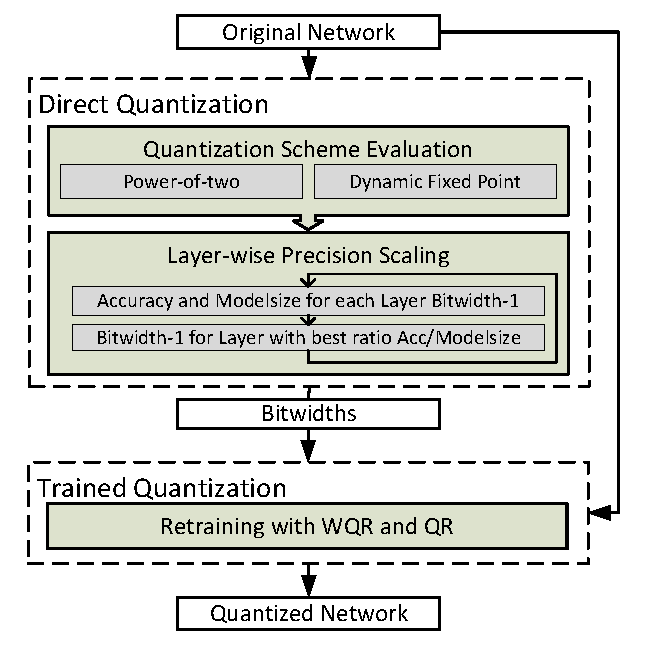
\includegraphics[width=\columnwidth]{img/process3.pdf}
\caption{Learned Weight Quantization step by step}\label{fig:process}
\end{figure}

While the first two steps serve for finding the best quantization method and 
bit-width for each layer when applying quantization without retraining, 
in the third step we perform retraining aiming to reduce the accuracy loss 
caused by quantization. In our flow, the weights are not first quantized and 
then retrained, but we always start from the high accuracy model, fine-tune 
weights with modified loss-functions and then perform quantization. This 
approach has the advantage that the network parameters are trained in full
precision but with the additional regularization terms which cause the weights 
to reduce their distance to the desired quantization levels before performing 
the actual quantization step. To better distinguish we use the term direct 
quantization for quantization without any fine-tuning. Trained quantization on the other hand consists of fine-tuning, followed by the actual quantization step. 
Input for the quantization process is a Deep Neural Network (DNN) $M$ with $N$ 
convolutional and/or fully connected layers and weight-tensors $W_n, 0<n<N$ of 
arbitrary resolution. Details on the network used for evaluation can be found in 
table \ref{tab:allconv}. Table \ref{tab:variables} summarizes the list of 
variables used in this work.

\begin{table}[ht!]
  \caption{Variables used in this work}
  \label{tab:variables}
  \begin{tabular}{ccl}
    \toprule
    	\textbf{Variable}&\textbf{Comment}\\
    \midrule
 		$M$& Original network model\\
		$M_q$ & Quantized network model\\
 		$N$& Number of layers\\
		$W_n$ & Original Weights\\
		$W_{q_n}$ & Quantized weights\\
		$b_n$ & Bit-widths for layers $n = 0...N$\\
		$Q_n$ & Quantization schemes for layers $n = 0...N$\\
		$Q_{p2}$ & Power-of-2 quantization scheme\\
		$n_1$ & Maximum exponent for Power-of-2 quantization\\
		$n_2$ & Minimum exponent for Power-of-2 quantization\\
		$s$ & Maximum absolute weight within the selected layer\\
		$Q_{dfp}$ & Dynamic Fixed Point quantization scheme\\
		$B$ & Unscaled Dynamic Fixed Point quantization scheme\\
		$acc_M $ & Classification accuracy of the original network\\
		$acc_{M_q} $ & Classification accuracy of the quantized network\\
		$\Delta acc $ & Accuracy degradation due to quantization\\
		$W_{mem} $ & Weight memory bits\\
		$\lambda_1 $ & Quantization-Regularization scale factor\\
		$QR $ & Quantization-Regularization Term\\
		$\lambda_2 $ & Weighted Quantization-Regularization scale factor\\
		$WQR $ & Weighted Quantization-Regularization term\\
  \bottomrule
\end{tabular}
\end{table}

%Aiming at hardware friendly implementation, in contrast to other works (e.g. \cite{Zhou2017a}) we absorb Batch-Normalization layers into the convolutional layers weights and biases, as they induce additional computational complexity and increase model size \cite{Ioffe2015}. This absorption can be performed without any performance degradation or retraining as Batch-Normalization merely presents a linear transformation to the input or output map of the preceding respectively succeeding layer. \todo[inline]{maybe add effect on number of computations and model size}

\subsection{Direct Quantization}
\label{subsec:quant}
In direct quantization, the original network $M$ is expressed as $M_q$ where 
the weights $W_n$ of each layer are represented as $W_{q_n}$. The values of 
$W_{q_n}$ are determined by rounding each element of $W_n$ to the quantization 
level with the smallest absolute distance of a previously defined quantization 
scheme $Q$.

\subsubsection{Quantization Scheme Evaluation}
Here, we present Power-of-two \cite{Zhou2017a} and Dynamic Fixed Point 
\cite{Hubara2016, Gysel2016a}, two different quantization schemes and 
compare their properties for direct and trained quantization.

\paragraph{Power-of-two quantization}
We implement Power-of-two (Po2) quantization similar as in \cite{Zhou2017a}. $Q_{p2}$ is given as
\begin{equation}\label{eq:pow2_quant}
Q_{p2} = \{\pm 2^{n_1},... ,\pm 2^{n_2},0\}.
\end{equation}
$n_1$ and $n_2$ are integers with
\begin{eqnarray}
n_1 &=& \lfloor log_2 \frac{4s}{3} \rfloor \label{eq:n1_max}\\
s &=&  max(abs(W)). \label{eq:s_max}
\end{eqnarray}
For a given bit-width $b$ and $n_2$ are defined by
\begin{equation}\label{eq:n2}
n_2 =  n_1 - (2^{b-1} -1).
\end{equation}

Thus, the quantization levels depend on the distribution of weights, 
especially on the weight with the highest absolute value. By adding `$0$' as 
a quantization level, we enable power-of-two quantization to also serve as a 
pruning mechanism when applied to weight matrices, as small weights are rounded 
to zero. In experiments symmetrical quantization schemes lead to higher 
classification accuracies for the quantized networks, 
therefore we only use $2^b-1$ of $2^b$ possible quantization levels.
%\cite{Zhou2017a}

\paragraph{Dynamic Fixed Point}
Dynamic fixed point (DFP) data type is successfully used in several works for either direct quantization or retrained model compression \cite{Hubara2016, Gysel2016a}.
For DFP quantization, we first define a set of $2^{b}-1$ equidistant quantization levels:
\begin{equation}\label{eq:dfp_nums}
B = \{\pm 2^{b-1}-1,\pm 2^{b-1}-2,... ,0\}.
\end{equation}
Similarly to Po2 quantization, we prefer a symmetric quantization scheme. 
Next $B$ is normalized and scaled, depending on the distribution of weights:
\begin{equation}\label{eq:dfp_quant}
Q_{dfp} = \frac{B}{2^{b-1}}*2^{n_1}.
\end{equation}

Figure \ref{fig:quant_hist} depicts the distribution of weights for an 
example layer of a CNN, before and after quantization. While 
figure \ref{fig:quant_hist}(a) shows the distribution for Po2 quantization, 
figure \ref{fig:quant_hist}(b) illustrates the distribution for DFP quantization. 
As can be seen that po2 has much irregular quantization values compared to DFP, 
and also considers the values close to `0' which might help to retain the 
information with lower weights and aid in improving the accuracy.


\begin{figure}[ht!]
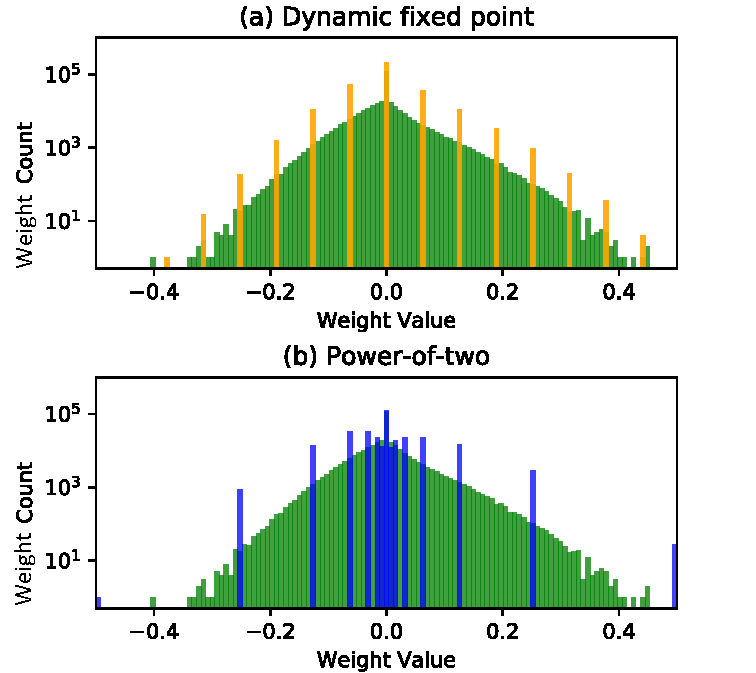
\includegraphics[width=\columnwidth]{img/histograms2.pdf}
\caption{Distributions before and after direct weight quantization for (a) Dynamic Fixed Point and (b) Power-of-two quantization}\label{fig:quant_hist}
\end{figure}

As accuracy degradation of the quantized model $M_q$ in comparison to the original model $M$ is a result of the quantization error, it is necessary to understand the relation between bit-width and quantization error for both datatypes.

With DFP quantization, the mean square error (MSE) can be reduced with 
increasing bit-width, since every additional bit divides the intervals in 
half (see fig. \ref{fig:quant_hist}a). 
Meanwhile when increasing bit-width in Po2 quantization, the new quantization levels are always added close to `0' (see fig. \ref{fig:quant_hist}b). As a consequence with Po2 quantization, the quantization error can only be reduced to a certain extent. Figure \ref{fig:quant_mse} shows the resulting mean square errors for one weight-tensor of an example layer when applying different bit-widths.

\begin{figure}[t]
%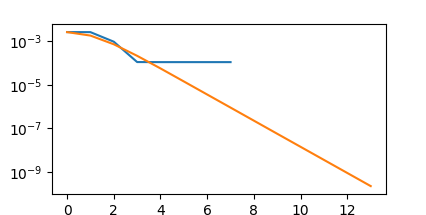
\includegraphics[width=\columnwidth]{img/MSE.PNG}
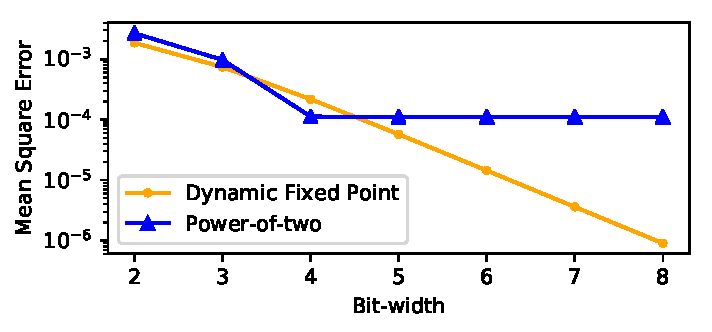
\includegraphics[width=\columnwidth]{img/mse.pdf}
\caption{Mean square error for an example layer when applying Power-of-two and Dynamic Fixed Point quantization with different bit-widths. While when using DFP quantization the error decreases exponentially, for Po2 quantization the quantization error reaches the minimum already at bit-width 4}\label{fig:quant_mse}
\end{figure}

In addition, we consider the amount of pruned weights as an important factor for model compression. In comparison to DFP, Po2 quantization decreases sparsity within the weight matrices as a result of quantization, due to the higher density of levels close to `0'. Therefore to fully benefit from the advantages of sparsity, an additional pruning step before retraining is recommended. In figure \ref{fig:quant_sparse} the number of pruned weights depending on the selected bit-width is shown for Po2 and DPF quantization.

\begin{figure}[t]
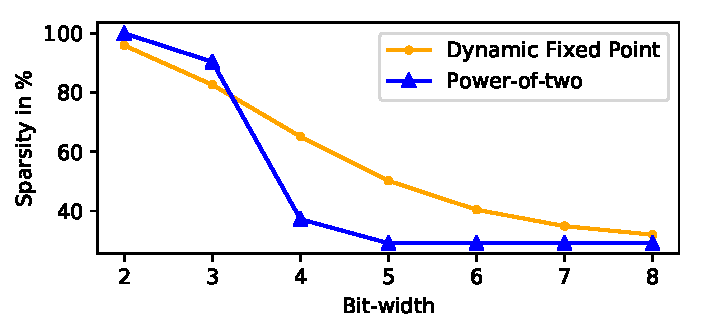
\includegraphics[width=\columnwidth]{img/sparse.pdf}
\caption{With increasing bit-widths the sparsity due to quantization decreases for Dynamic Fixed Point and Power-of-two quantization. Sparsity is denotes the amount of weights that are 0 relative to the total amount of Weights}\label{fig:quant_sparse}
\end{figure}

%AJ: I reformulated the following paragraph to make it clearer:
Figures \ref{fig:quant_mse} and \ref{fig:quant_sparse} suggest that for direct Po2 quantization bit-widths higher than 4-bit do not further decrease the $\Delta acc$ but 4-bits in comparison to 5-bits slightly increase sparsity. 
%Figures \ref{fig:quant_mse} and \ref{fig:quant_sparse} suggest that for direct Po2 quantization bit-widths higher than 4-bit cannot further decrease the resulting $\Delta acc$. Furthermore, since 4-bit Po2 in comparison to 5-bit Po2 increases sparsity, but does not significantly increase the MSE, we can suspect similar results in terms of accuracy but more pruned weights for 4-bit Po2. 
On the other hand, by scaling the bit-width of DFP the resulting MSE can be reduced exponentially (Fig. \ref{fig:quant_mse}) meaning that even bit-widths higher than 8 bit deliver more accurate results. In terms of sparsity, DFP prunes more weights than Po2 for bit-widths of four and higher.

Based on these observations we expect that for direct DFP quantization $\Delta acc$ can be reduced to almost 0, based on Layer-wise Precision Scaling. For direct Po2 quantization we expect a higher $\Delta acc$ and no significant increase of accuracy for bit-widths higher than five. It can be seen in figures \ref{fig:lw_scale} and \ref{fig:lw_100} that these expectations are confirmed.
%\caj{Are these expectations confirmed? If yes, let's point to the graph or section, where this is evident.}

\subsubsection{Layer-wise Precision Scaling}
\label{layerwise}
Secondly, to further reduce the model-size, we apply different quantization schemes per layer by optimizing bit-widths. In comparison to choosing equal bit-width for each layer, due to the varying amount of parameters and varying distribution of weights between layers, selecting fitting quantization schemes for each layer can enable lower bit-widths per layer without reducing the resulting accuracy.  For the experiments we assume either DFP or Po2 quantization. For an arbitrary network $M$ with accuracy $acc_{M}$ applying weight quantization with the set of bit-widths $b_n$ leads to accuracy $acc_{Mq}$
and weight memory bits\highlight{
\begin{equation}\label{eq:w_mem}
W_{\text{mem}} = \sum^N_n{\text{card}(W_n)*b_n}
\end{equation}
where $\text{card}(A)$ denotes the cardinality of set $A$.}
%AJ: Symbols with more than one letter are better typeset as\text{} in math mode.
For each $b_n$ we compute the resulting accuracy degradation
\begin{equation}\label{eq:acc_deg}
\Delta acc = acc_{M} - acc_{Mq}
\end{equation}
and iteratively decrease the bit-width of the layer where a lower bit-width leads to the smallest product of $\Delta acc * W_{mem}$  (see algorithm~\ref{alg:lw}).

\begin{algorithm}
\caption{Layer-wise Precision Scaling}\label{alg:lw}
\begin{algorithmic}
\State 
\Procedure {Layer-wise Precision Scaling}{$M$}
	\State initialize $b_n$
	\While{$\Delta acc < \epsilon$}
		\ForAll{$n$ in layers}	
			\State bitwidth of $layer_n$ - 1
			\State Compute $Acc_{M_q}$, $\Delta acc$ and $W_{mem}$
			\State bitwidth of $layer_n$ + 1
		\EndFor	
		\State Decrease bitwidth of layer with smallest $\Delta acc * W_{mem}$
	\EndWhile
\EndProcedure
\end{algorithmic}
\end{algorithm}
Figure \ref{fig:lw_scale} shows the results for Layer-wise Precision Scaling performed by algorithm \ref{alg:lw} on All-Convolutional Network \cite{Springenberg2015} for CIFAR-10. We can deduce that while DFP quantization also allows direct quantization, whereas for power-of-two quantization almost always an additional fine-tuning step is necessary to achieve high accuracy results.

\begin{figure}[t]
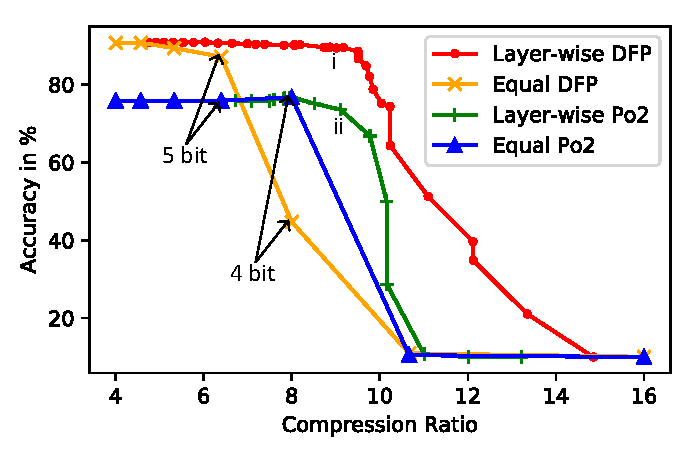
\includegraphics[width=\columnwidth]{img/layerwise.pdf}
\caption{Layer-wise Precision Scaling compared with equal bit-width quantization for DFP and Po2 quantization. Compression ratio is the ratio between 32bit weight memory and the weight memory for the quantized network. Point i indicates DFP with $b_n=\lbrack$7 7 7 4 4 3 3 7 7$\rbrack$ , point ii indicates Po2 with $b_n=\lbrack$4 4 4 4 3 3 4 4 4$\rbrack$.}\label{fig:lw_scale}
\end{figure}

\subsection{Trained Quantization}
The used datasets (CIFAR-10, CIFAR-100 and SVHN) are already divided into \textbf{test data} and \textbf{training data}. While with Layer-wise Precision Scaling as described in section \ref{layerwise} focuses on decreasing $\Delta acc * W_{mem}$ without retraining, we can additionally reduce $\Delta acc$ by retraining the original network on the training data with the goal of increasing accuracy of the classifier on test data. As a consequence we use the performance metrics in table \ref{tab:metrics}.
\begin{table}[ht!]
  \caption{Performance Metrics used for Fine-tuning}
  \label{tab:metrics}
  \begin{tabular}{ccc}
    \toprule
    	\textbf{Variable}&\textbf{Metrics}&\textbf{Comment}\\
    \midrule
 		$acc_{tr}$&Training Accuracy& Accuracy of the network\\
 		&&  on the training data\\
		$acc_M$&Test Accuracy & Accuracy of the  network \\
 		&&  on the test data\\
		$acc_{M_q}$&Quantized & Accuracy of the network \\
		&Test Accuracy\footnotemark& with quantized weights\\
		&& on the test data\\
		$acc_{init}$&Init. Quantized & Accuracy of the network \\
		&Test Accuracy& with direct quantized initial\\
		&&weights on the test data\\
		CR& Compression Ratio & Ratio $W_{Mem}$ of original model\\
		& & to $W_{Mem}$ of quantized model\\
  	\bottomrule
\end{tabular}
\end{table}
\footnotetext{For the computation of Quantized Test Accuracy, the weights of the network are directly quantized after each epoch.}

\subsubsection{Quantization-Regularization}
\label{subsec:qr}
To decrease $\Delta acc$ for a selected set of bit-widths $b_n$, we need to find the best set of $W_n$ so that approximation with $Wq_n$ achieves a maximum of $acc_{Mq}$. As shown in \cite{Lin2015a, Shin2017} the degradation of classification accuracy of a DNN due to quantization is directly related to the signal to quantization-noise ratio (SQNR) and the amount of weights per layer, as both influence the SQNR of the intermediate layer outputs and as a consequence the resulting network outputs. Therefore retraining network weights to achieve lower SQNR without reducing $acc_{M}$, leads to an increased accuracy of the quantized network.
To enforce weight quantization during the training phase we define the quantization-regularization (QR) term as\highlight{
\begin{equation}\label{eq:quant_reg}
QR = \sum^{N}_{n}\sum^{\text{card}(W_n)}_{i}\frac{\mid W_{n_i}-Wq_{n_i}\mid}{\max(Q_n)*\text{card}(W_n)}
\end{equation}
 }
which expresses the mean of the absolute weight distances of each weight to the corresponding quantized value.

By adding the QR-term to the loss function (eq. \ref{eq:lossfunction}) weights are forced closer to the quantization levels during retraining.
\begin{equation}\label{eq:lossfunction}
\textrm{Modified Loss = Loss}+\lambda_1*QR
\end{equation}
During fine-tuning with the parameter $\lambda_1$ the trade-off between $min(Loss)$ and $min(QR)$ and, as a consequence, between $min(\Delta accuracy)$ and $max(acc_{M})$ can be adjusted. For the experiments we applied fixed $\lambda_1$ and linearly increasing $\lambda_1$ (e.g. $\lambda_1=10*epoch$). Figure \ref{fig:weightreg} depicts the trained quantization process. With each epoch the weights are pulled closer to the quantization levels, thus decreasing $QR$ and $\Delta acc$.

\begin{figure}[ht!]
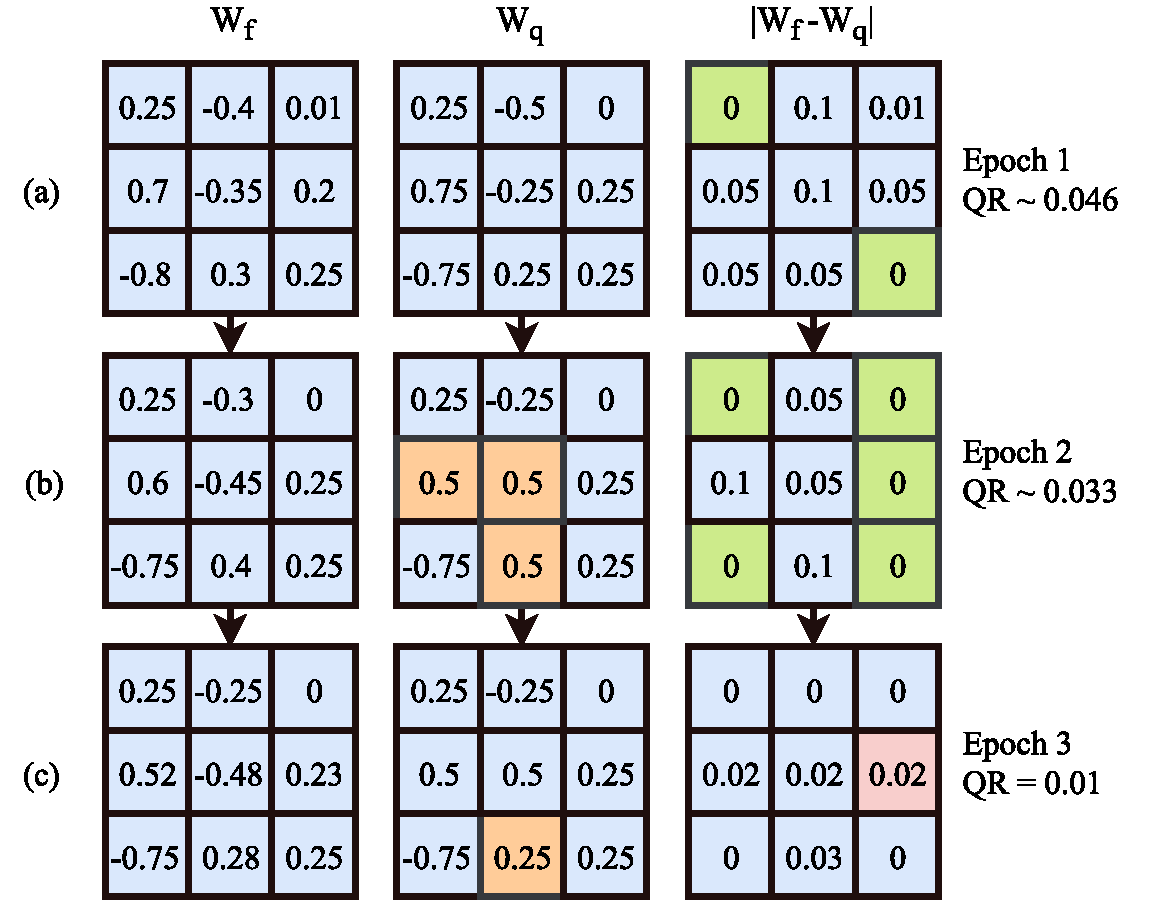
\includegraphics[width=\columnwidth]{img/weightreg.pdf}
\caption{Illustration of Quantization-Regularization. The first column shows the floating point values of the weights on which the actual training is performed. The second column shows the quantized weights, and the third column the element-wise absolute difference of floating point and quantized weights. Changes of quantized weights are marked in the second column. \highlight{Weight update for $W_f$ is performed based on backpropagation of the modified loss function (eq. \ref{eq:lossfunction}).} Successfully quantized weights are marked in the third column. After Epoch 1 (a) the weights are hardly regularized and $QR$ is relatively large. Epoch 2 (b) shows that due to regularization, weights are pulled closer to the quantization levels $\mathbf{Q_n=\{0,\pm 0.25, \pm 0.5, \pm 0.75\}}$ and $QR$ gets smaller. For three of the weights the resulting quantization level changed, and weights decrease their distance to the next quantization level. Epoch 3 (c) shows further reduction of the $QR$ term.}\label{fig:weightreg}
\end{figure}

While choosing a high ($>1000$) $\lambda_1$ leads to fast quantization with strong accuracy degradation, a low $\lambda_1$ value ($<1$) does not enforce quantization. Either way, much like weight decay low $\lambda_1$ values can help avoiding overfitting during training.

\subsubsection{Weighted Quantization-Regularization}
\label{subsec:wqr}
While in normal QR each weight within one layer is considered equally important for reaching high classification accuracy, the efficiency of pruning \cite{Han2015a,Yang2017,Dong2017} shows that especially weights with small magnitudes can be changed without reducing the accuracy of the network.
Similarly to \cite{Zhang2015}, the weights can be divided into two disjoint subsets, where QR is applied on one of the subsets while the other weights are being retrained without QR. Going one step further we can multiply the QR value of each weight with the absolute magnitude of the weight.
\footnote{Previously the sum of weights is normalized to 1 for each layer}
This strategy forces quantization stronger on weights with higher magnitudes which can be especially useful for Po2 quantization, where density of quantization levels decreases with increasing weight values. Therefore we define the Weighted Quantization-Regularization (WQR) term as\highlight{
\begin{equation}\label{eq:w_quant_reg}
WQR = \sum^{N}_{n}\sum^{\text{card}(W_n)}_{i}(\frac{\mid W_{n_i}-Wq_{n_i}\mid\mid W_{n_i}\mid}{\max(Q_n)^2*\text{card}(W_n)}
\end{equation}}
and similarly to equation \ref{eq:lossfunction} we can weight the trade-off between accuracy and weight regularization with $\lambda _1$ and $\lambda _2$ (eq. \ref{eq:lossfunction2})

\begin{equation}\label{eq:lossfunction2}
\textrm{Modified Loss = Loss} + \lambda _1 *QR + \lambda _2 *WQR
\end{equation}

Again during training the parameters $\lambda_1$ and $\lambda_2$ have to be adjusted carefully to reach the desired improvement of $Acc_{Mq}$, without at the same time decreasing $Acc_{M}$. In our experiments we found a linear increasing $\lambda_2$ to work best (e.g. $\lambda_2 = 10*\textrm{epoch}$).

For fine-tuning, we use algorithm \ref{alg:quant}.

\begin{algorithm}[ht!]
\caption{Fine-tuning with Quantization-Regularization and Weighted Quantization Regularization}\label{alg:quant}
\begin{algorithmic}
\State 

\Procedure {Trained Quantization}{$M$, $b_n$, $\lambda_1$, $\lambda_2$}
	\For{epochs}
		\ForAll{Mini Batches} \Comment{Train on Training Data}
			\For{$n >= N$}	\Comment{Quantize all Layers}
				\State $Q_n(W_n,b_n)$ \Comment{Determine Quantization Scheme}	
				\State $W_{q_n}$ = Quantize($W_n$,$Q_n$) \Comment{Quantize Weights}		
			\EndFor
			\State Loss + $\lambda_1*QR(W_n, Q_n, W_{q_n}) + \lambda_"*WQR(W_n, Q_n, W_{q_n})$
			\State Backpropagation(Loss,QR,WQR,$\lambda_1$,$\lambda_1$)		
		\EndFor	
		\State Compute $Acc_{M}$	\Comment{Test Accuracy}
		\State Compute $Acc_{M_q}$	\Comment{Quantized Test Accuracy}
	\EndFor
	\State \textbf{return} $M_q$	\Comment{Return Quantized Model}
\EndProcedure
\end{algorithmic}
\end{algorithm}


Figure \ref{fig:acc_example} illustrates the fine-tuning process for 4-bit equal bit-width Po2 quantized All-Convolutional Net for CIFAR-10. At the beginning of the fine-tuning process the term $\lambda_2*WQR$ increases due to the increasing $\lambda_2$ value, while the $WQR$-Term decreases exponentially. At Epoch 200 learning rate is decreased from $1e^{-4}$ to $1e^{-5}$ leading to the drop of $\lambda_2*WQR$. This can be explained by fact that a larger learning rate leads to larger weight changes. If the weights are already close to the quantization levels a lower learning rate can lead to better approximation of the weights to the quantization levels.
\begin{figure}[ht!]
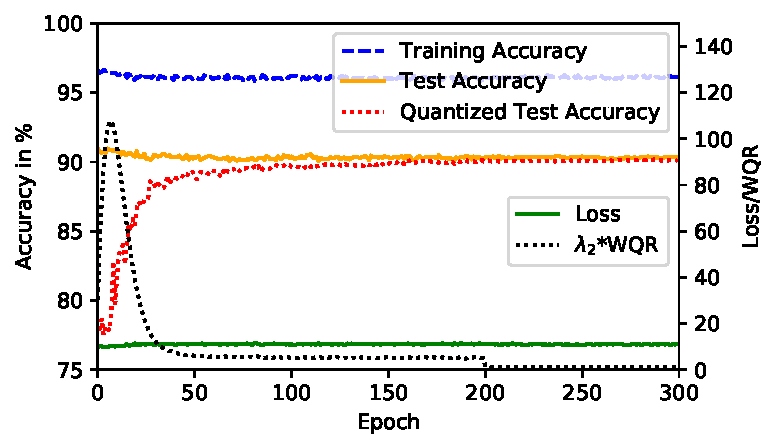
\includegraphics[width=\columnwidth]{img/accuracy.pdf}
\caption{Fine-tuning of All-Convolutional Net for CIFAR-10 with linear increasing $\pmb{\lambda}\mathbf{_2}$ for 4-bit equal bit-width Po2 quantization. $\pmb{\Delta}\mathbf{Acc}$ is decreased from $\mathbf{14.09\%}$ to $\mathbf{0.14\%}$ resulting in Quantized Test Accuracy of $\mathbf{90.18\%}$ in comparison to initial Floating Point Test Accuracy $\mathbf{90.83\%}$.}
\label{fig:acc_example}
\end{figure}




%Adaptive methods give a good idea of how models can be approximated by simply transforming them, but when retraining the question is how to choose the best bitwidth per layer. We can use quantization-regularization and observe how the weights get closer to the quantization levels. If the MSE stays big for one layer, that basically means, that the bitwidth for that layer should be approximated with a higher precision.


\subsection{Summary and Analysis}
In combination, the discussed techniques for quantization (sec.~\ref{subsec:quant}), Layer-wise Precision Scaling (sec.~\ref{layerwise}) and fine-tuning with QR (sec.~\ref{subsec:qr}) and WQR (sec.~\ref{subsec:wqr}) facilitate DNN weight compression.

The above discussed two quantization schemes behave differently during the quantization process and require different quantization strategies. For bit-widths higher than 7 bit DFP can be applied without any retraining and still achieves almost floating point accuracy. For equal bit-width DFP quantization with 7 bit and less, $\Delta acc$ increases and fine-tuning is necessary to reach the accuracy of the original network. On the other hand Po2 quantization always requires retraining, as even the use of bit-widths higher than five reduce the quantization error only to a certain extent.

To increase the compression ratio when applying DFP quantization, layer-wise precision scaling is an effective method, since not all layers require the same the bit-width for high accuracy. For instance, in modern convolution-only networks, layers with fewer parameters require larger bit-widths~\cite{Lin2015a}. As a result, when applying layer-wise precision scaling the weights of the output and input layers are kept at high precision, as they usually have the fewest parameters.
In comparison to DFP, for Po2 quantization, layer-wise precision scaling does not proof to be as effective, as almost the same bit-width is recommended throughout the network to achieve best accuracy.

\begin{figure}[ht!]
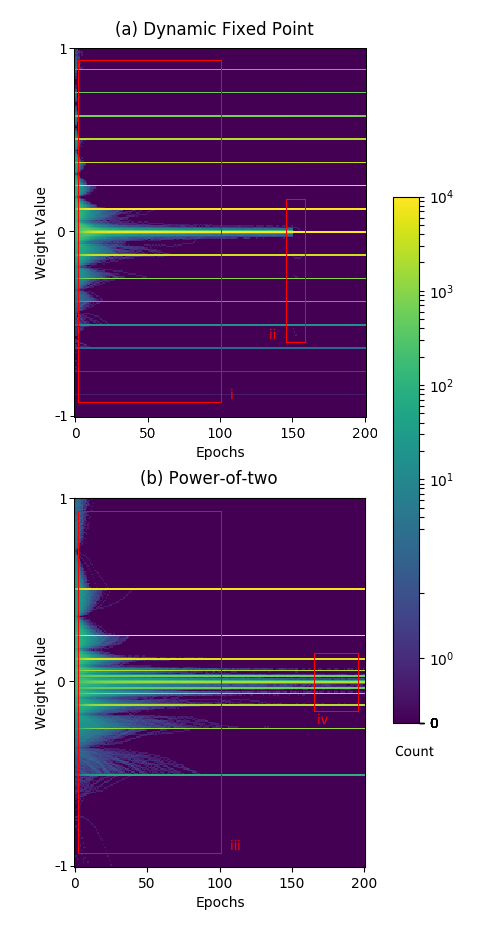
\includegraphics[width=\columnwidth]{img/histotime2.png}
\caption{Distribution of weights in layer 5 of AllConvNet (CIFAR-10) during fine-tuning with WQR and QR to (a) 4-bit Dynamic Fixed Point and (b) 4-bit Po2. DFP (a) is trained with $\mathbf{\lambda_2 = epoch*10}$. Region i shows the faster quantization of weights with high magnitudes and slower quantization of weights close to 0. At epoch 150 QR is applied with $\mathbf{\lambda_1 = 100}$ to quantize also weights with smaller values (ii). Po2 (b) is trained with $\mathbf{\lambda_2 = epoch*10}$. Region iii also shows slower quantization for small magnitude weights. Due to the distribution of quantization levels, weights around 0 are already close to the next quantization level (iv).}
\label{fig:WQR_QR}
\end{figure}

For fine-tuning of Po2 and DFP quantized networks, QR and WQR can be added to the loss function as regularization terms to force quantization during retraining. While the QR term forces all weights equally to reduce the distance to the next quantization level, the WQR term is reduced for weights with small magnitudes. Therefore, WQR operates less restrictive than QR, as the original QR value is multiplied with a factor from 0 to 1 (normalized weight magnitude). As a consequence it is an effective strategy to apply WQR followed by QR fine-tuning.

Figure \ref{fig:WQR_QR} shows the distribution of weights in layer 5 during (a) 4-bit DFP and (b) 4-bit Po2 quantization of the All-Convolutional Network for the CIFAR-10 dataset. For fine-tuning to 4-bit DFP quantization (Fig.\ref{fig:WQR_QR}a) $\lambda_2$ is increased linearly by a factor of 10 with each epoch. As QR scale factor $\lambda_1$ we use 0 before and 100 starting at epoch 150. Region i in figure \ref{fig:WQR_QR}a shows the decelerated quantization of small magnitude weights. Starting with epoch 150, also weights close to 0 are quantized, due to the application of QR (Fig. \ref{fig:WQR_QR}a,ii). For 4-bit Po2 quantization only WQR is necessary ($\lambda_2 = epoch*10$) to achieve quantization. Due to the the non-equidistant distribution of quantization levels in Po2 quantization, the weights with high magnitudes take longer than in DFP quantization to reach the quantization levels (Fig. \ref{fig:WQR_QR}b,iii). Additional QR is not necessary since, due to the high density of quantization levels close to 0, the weights with smaller magnitudes induce a very small quantization error (Fig. \ref{fig:WQR_QR}b,iv).

QR and WQR enable trained quantization to improve performance in comparison to direct quantization. Regularization-based quantization is very simple to implement and applicable for any quantization scheme. As a consequence QR and WQR could be employed alongside other effective quantization techniques such as stochastic quantization. Besides the simplicity of the approach, it also allows a deeper analysis of quantization schemes by recording the change of weight distribution during training.

While enabling compression for more efficient inference, during training QR and WQR add overhead due to the mandatory quantization step after each mini-batch and the necessary computations for calculation of QR and WQR. The fact that all weights have to be stored as floating point values and quantized values, increases the weight memory during training by a factor of 2.

%Since the number of weights in state-of-the-art DNNs is smaller by at least the factor 100 than the MACs required for one feed forward computation, we can neglect this disadvantage. 



\section{Experimental Results}
The following section describes the experimental results for direct and trained quantization of All-CNNs on three datasets.

\subsection{Experimental Setup}
For experimental evaluation, we apply the proposed methods on All-Convolutional Networks for the Datasets CIFAR-10 \cite{Krizhevsky2009}, CIFAR-100 and SVHN \cite{netzer2011reading}. We use All-Convolution Network model All-CNN-C from \cite{Springenberg2015} for evaluation. The CNN Architecture summed up in table \ref{tab:allconv} consists of nine convolution layers and a global average pooling layer. Due to the similar filter-width and height the number of weights in the convolution layers mainly depends on the filter-depths. The number of operations also depends on the layer-output dimensions. However, it needs to be 
noted that the proposed technique is neither architecture nor dataset bound. 

\begin{table}[ht!]
  \caption{All-CNN-C Architecture and the number of weights and MAC-operations for one forward computation with batch-size one.}
  \label{tab:allconv}
  \begin{tabular}{c|c|c|c}
    \toprule
    	\textbf{Layer (WxH) }& \textbf{Output Dim. (WxHxD) }& \textbf{\#Weights} & \textbf{\#MACs} \\
    \midrule
    	Input &  32x32x3 & - & - \\
    	Conv. 3x3 &  32x32x96 & 2K & 2.3M \\
    	Conv. 3x3 &  32x32x96 & 83K & 74.6M\\
    	Conv. 3x3 &  32x32x96 & 83K & 74.6M\\
    	Pooling 2x2 &  16x16x96 & - & -\\
    	Conv. 3x3 &  16x16x192 & 165K & 32.5M\\
    	Conv. 3x3 &  16x16x192 & 332K & 65M\\
    	Conv. 3x3 &  16x16x192 & 332K & 65M\\
    	Pooling 2x2 &  8x8x192 & - & -\\
    	Conv. 3x3 &  8x8x192 & 332K & 11.9M\\
    	Conv. 1x1 &  8x8x192 & 37K & 2.4M\\
    	Conv. 1x1 &  8x8x10 & 2K & 0.1M\\
    	Pooling 8x8 &  10 & - & -\\
            \midrule
    	\textbf{Total}&  - & \textbf{1386K} & \textbf{329.7M} \\
  \bottomrule
\end{tabular}
\end{table}

For the three datasets, we use the predefined training and test sets. For the floating point baselines we trained the CNN for 350 epochs with initial \highlight{learning rate $10^{-3}$} multiplied by a fixed multiplier after epochs 200 and 300. To avoid over-fitting, we use dropout with dropout rate 0.5 after layers. In contrast to the original All-CNN paper \cite{Springenberg2015}, the models are not regularized by weight decay to avoid interfering with the studied regularization methods. In terms of data augmentation we only apply horizontal flipping and random shifting by a maximum of 3 pixels. 

\subsection{Performance Analysis}
We evaluate the performance of the proposed method comparing the test accuracy of the original network with the resulting accuracies after direct and trained quantization. For the tables \ref{tab:res_CIFAR10}, \ref{tab:res_CIFAR100} and \ref{tab:res_SVHN}, we make use of the abbreviations in table \ref{tab:metrics}.
We aim to achieve high compression rates in terms of weight memory while maintaining high test accuracy. \highlight{In addition to bit-width reduction we also consider the resulting sparsity as an important factor for possible further compression.} Assuming skipping of multiplications with 0 weights, sparsity also reduces the amount of required MAC-operations for forward computation.\footnote{The number of skipped MACs due to a pruned weight depends on the layer-input dimensions. Therefore sparsity in weights is unequal to sparsity in MACs.} \highlight{For all experiments except the two marked, bit-width for activations is 32-bit Fixed Point}.
%\caj{Why is the sparsity of weights different from the sparsity of MACs in the tables?}
%\cmw{This derives from the reuse of weights and the input dimensions. Say in layer 1 a weight is 0, it accounts for 32x32 multiplications, while a weight in layer 5 for 16x16 multiplications.}
%\todo[inline]{
%comparison to other methods (improvement)}
%\todo[inline]{Results like in IMAGE shown implementing the SQNR and then Retraining (necessity of the approach)
%\newline comparison to other methods (improvement)
%\newline Relationship Accuracy, Loss during retraining
%\newline influence of the lambda parameter
%\newline influence of learning rate
%}




\subsubsection{CIFAR-100}


CIFAR-100 is an image classification dataset consisting of a training set of 50000 and a test set of 10000 32$\times$32 color images representing 100 different categories such as airplanes, automobiles, birds, cats, deers,dogs, frogs, horses, ships and trucks \cite{Krizhevsky2009}. The training batches contain exactly 5000 images from each class. Table \ref{tab:res_CIFAR10} shows the resulting accuracies after fine-tuning with 200 epochs of WQR with $\lambda_2 = epoch\times 10$. In addition $\lambda_1$ is set to 100 starting at epoch 150. This setup is not optimal for all configurations, as in some cases training with only QR would be sufficient, but it allows using the same parameterization for each iteration increasing comparability. Compared to a full implementation (32-bit), the proposed layer-wise quantization (DFP-lw) saves $\sim$4-8$\times$ in terms of weight memory and has an accuracy loss by $\sim$0.1-4.5\%. Compared to the reduced equal bit-width quantization, the proposed layer-wise quantization has higher sparsity and smaller weight memory. 

\begin{table*}[ht!]
\caption{Results in comparison to floating point baseline of All-CNN for CIFAR-100 (CR=Compression ratio)}
%  \caj{Is the activation bit-width 8bit for all experiments? If yes, we should write this; if not, we should explain what the activation bit-width is in those cases. Anyway, the footnote is the wrong place to explain this. }
%  \cmw{Added explanation in first paragraph section 4.2}
  \label{tab:res_CIFAR100}
  \begin{tabular}{cc|ccc|cc|ccc}
\toprule
    	$b_n$&Type&$W_{mem}$\lbrack$Bit$\rbrack$$&CR& Sparsity$\lbrack\%\rbrack$ & non-0 MACs & MAC Sparsity$\lbrack\%\rbrack$ & $acc_{tr}\lbrack\%\rbrack$ & $acc_{init}\lbrack\%\rbrack$ & $acc_{M_q}\lbrack\%\rbrack$\\
\hline
 		32 bit & float & 44344K & 1 &  0 & 329.7M & 0 & 83.24 & 63.03 &  \textbf{63.03} \\
\hline
 		8 bit & DFP-eq & 11086K & 4 & 5.8 & 304.8M & 7.6 &83.5&62.43&\textbf{62.99} \\
 		7 bit & DFP-eq & 9700K & 4.6 & 11.5 & 280.3M & 15 &82.65&61.86&\textbf{62.38}\\
 		6 bit & DFP-eq & 8314K & 5.3 & 21.9 & 234.1M & 29 & 81.02&58&\textbf{61.19}\\
 		5 bit & DFP-eq & 6928K & 6.4 & 38.9 & 161M & 51.2 & 76.99&43.72&\textbf{59.54}\\
\hline
       	$\lbrack$9	9	9	9	6	5	7	9	9$\rbrack$ & DFP-lw & 9485K & 4.7 & 14.6 & 289.5M & 12.2 &83.44&62.90&\textbf{62.93}\\
       	$\lbrack$9	9	9	9	5	5	5	9	9$\rbrack$ & DFP-lw & 8490K & 5.2 & 23.2 & 279.2M & 15.3 &82.45&62.45&\textbf{62.64}\\
       	$\lbrack$9	9	9	5	4	4	5	9	9$\rbrack$ & DFP-lw & 7163K & 6.2 & 36.4 & 243.4M & 26.2 &80.76&61.70&\textbf{62.29}\\ 	
        $\lbrack$9	6	5	5	3	3	4	7	9$\rbrack$ & DFP-lw & 5513K & 8.0 & 60.4 & 133.6M & 59.5 &73.76&55.69&\textbf{58.58}\\
\hline
 		4 bit & Po2-eq & 5543K & 8 & 18.3 & 255.2M & 22.6 & 79.47 & 51.27 & \textbf{60.94}\\
\hline
\end{tabular}
\end{table*}

\begin{table*}[ht!]
  \caption{Results in comparison to floating point baseline of All-CNN for CIFAR-10}
  \label{tab:res_CIFAR10}
  \begin{tabular}{cc|ccc|cc|ccc}
\hline
    	$b_n$&Type&$W_{mem}\lbrack$Bit$\rbrack$&CR& Sparsity$\lbrack\%\rbrack$ & non-0 MACs & MAC Sparsity$\lbrack\%\rbrack$ & $acc_{tr}\lbrack\%\rbrack$ & $acc_{init}\lbrack\%\rbrack$ & $acc_{M_q}\lbrack\%\rbrack$\\
\hline
 		32 bit & float & 43791K & 1 & 0 & 329.7M & 0 & 96.69 &  90.83 &  \textbf{90.83} \\
\hline
 %		all 5 bit & DFP & 6842K & 6.4 & 27.4 & 185.9M & 43.4 & 95.82 & 87.13 & \textbf{89.92}\\
  		8 bit & DFP-eq\footnotemark & 10947K & 4 & 4.2 & 303.5M & 7.6 & 96.64 & 90.65 & \textbf{90.85}\\
 		4 bit & DFP-eq & 5474K & 8 & 42.3 & 140.7M & 57.2 & 94.4 & 44.47 & \textbf{88.63}\\
\hline
              	$\lbrack$8 8 8 5 4 4 3 8 8$\rbrack$ & DFP-lw$^4$ &5929K& 7.38& 36.8 & 243M & 26 & 96.49 & 90.14 &\textbf{90.81}\\
              	$\lbrack$7 7 7 4 4 3 3 7 7$\rbrack$ & DFP-lw &5432K& 8.1&46.1&203.9M&37.9&96.01&90.07&\textbf{90.32}\\
 %		$\lbrack$6 6 4 4 3 3 3 5 6$\rbrack$ & DFP &4690K& 9.3&57.2&126.6M&61.4&95.16&87.79&\textbf{89.53}\\

 %		5 bit & Po2 & 6842KBit  & 6.4 & 0 & 327.8M & 0.01&96.22&90.45&75.56&\textbf{90.21}\\
 \hline
 		4 bit & Po2-eq & 5474K & 8 & 13.2 & 255.9M &  22.1 &96.13&76.73&\textbf{90.18}\\
 %		all 5 bit & DFP & 6842K & 6.4 & 27.4 & 185.9M & 43.4 & 95.82 & 87.13 & \textbf{89.92}\\
\hline
\end{tabular}
\end{table*}

\begin{table*}[ht!]
  \caption{Results in comparison to floating point baseline of All-CNN for SVHN}
  \label{tab:res_SVHN}
  \begin{tabular}{cc|ccc|cc|ccc}
\hline
    	$b_n$&Type&$W_{mem}\lbrack$Bit$\rbrack$&CR& Sparsity$\lbrack\%\rbrack$ & non-0 MACs & MAC Sparsity$\lbrack\%\rbrack$ & $acc_{tr}\lbrack\%\rbrack$ & $acc_{init}\lbrack\%\rbrack$ & $acc_{M_q}\lbrack\%\rbrack$\\
\hline
 		32 bit & float & 43791K & 1 & 0 & 329.7M & 0 & 97.70 & 95.84 & \textbf{95.84} \\
\hline
% 		all 5 bit & DFP & 6842K & 6.4 & 27.4 & 185.9M & 43.4 & 95.82 & 87.13 & \textbf{89.92}\\
 		4 bit & DFP-eq & 5474K & 8 & 43.5 & 166.8M & 49.2 & 96.27 & 86.17 & \textbf{95.37}\\
\hline
  %     	$\lbrack$7 7 6 4 3 3 4 7 6$\rbrack$ & DFP-lw &5347K& 8.2&54.1&190.9M&41.8&96.69&95.57&\textbf{95.89}\\
 		$\lbrack$6 4 4 3 3 3 4 5 6$\rbrack$ & DFP-lw &4690K& 9.3&62.7&126.6M&63.2&96.43&95.03&\textbf{95.89}\\
         $\lbrack$5 4 4 3 3 3 3 3 3$\rbrack$ & DFP-lw &4276K& 10.23&70.5&116.7M&64.4&95.52&89.86&\textbf{95.36}\\
\hline
 %		5 bit & Po2 & 6842KBit  & 6.4 & 0 & 327.8M & 0.01&96.22&90.45&75.56&\textbf{90.21}\\
 		4 bit & Po2-eq & 5474K & 8 & 17.0 & 272.8M & 16.9  &97.02&91.93&\textbf{96.02}\\
\hline
\end{tabular}
\end{table*}



In addition, figure \ref{fig:lw_100} depicts the results of trained quantization in comparison to direct quantization. We can see that retraining with QR and WQR in all cases increases classification accuracy in comparison to direct quantization.

\begin{figure}[ht!]
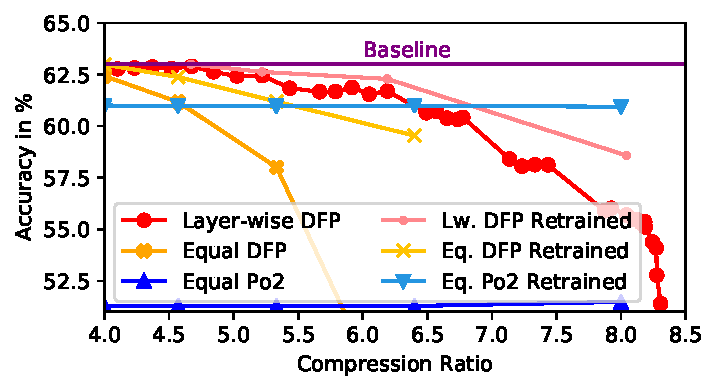
\includegraphics[width=\columnwidth]{img/res100.pdf}
\caption{Results for direct and trained DFP and Po2 quantization with equal bit-widths on ALL-CNN for CIFAR-100. For DFP also Layer-wise Precision Scaling with direct and trained quantization is illustrated.}\label{fig:lw_100}
\end{figure}
Comparing equal bit-width quantization with Layer-wise Precision Scaling for DFP datatype, we can see that for similar compression ratios, equal bit-width (DFP-eq) never reaches the accuracy of Layer-wise Precision Scaling (DFP-lw), even when retraining with WQR/QR is applied. For Po2 quantization we found equal 4 bit quantization (Po2-eq) the most effective method as higher bit-widths did not increase accuracy and Layer-wise Precision Scaling for lower than 4 bit leads to drastic accuracy drop.


\subsubsection{CIFAR-10}
CIFAR-10 is a benchmark image classification dataset equal to CIFAR-100 in terms of image and dataset sizes, which instead of 100 classes divides the images into 10 classes. We use the same training method as for CIFAR-100. The results for trained quantization of All-CNN for CIFAR-10 are shown in table \ref{tab:res_CIFAR10}. To allow comparing to other works for the two marked configurations, we also quantized the activations to 8-bit DFP. In contrast to ALL-CNN for CIFAR-100, for this dataset higher compression rates can be achieved. For Compression Ratio $\sim 8$, DFP with Layer-wise Precision Scaling (DFP-lw) gives lowest accuracy degradation of $0.51$ percentage points. For equal bit-with quantization Po2 outperforms DFP by $1.55$ percentage points. For Compression Ratio $7.38$ classification accuracy of DFP with Layer-wise Precision Scaling is only $0.01$ percentage points below the floating point baseline.

\begin{figure}[ht!]
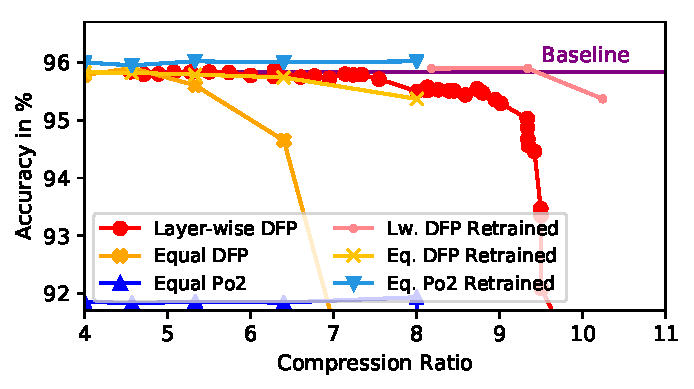
\includegraphics[width=\columnwidth]{img/ressvhn.pdf}
\caption{Results for direct and trained DFP and Po2 quantization with equal bit-widths on ALL-CNN for SVHN. For DFP also Layer-wise Precision Scaling with direct and trained quantization is illustrated.}\label{fig:lw_svhn}
\end{figure}
\subsubsection{SVHN}
The SVHN image classification dataset consists of 694K 32$\times$32 color images for training and 26K images for testing. The images represent digits form 0 to 9.
Similarly to CIFAR-100 and CIFAR-10 we perform Layer-wise Precision Scaling and retraining with WQR and QR for model compression. The results are shown in table \ref{tab:res_SVHN} and figure \ref{fig:lw_svhn}. For the SVHN dataset at Compression Ratio $\sim 8$, Po2 quantization and DFP with Layer-wise Precision Scaling both outperform the original baseline model.

\vspace{1ex}
Comparing the results for the datasets CIFAR-100, CIFAR-10 and SVHN, we can conclude that the attainable Compression Ratio for lossless trained quantization with QR/WQR not only depends on the selected datatype and bit-widths, but also on the selected datasets. 
\highlight{While for CIFAR-10 and SVHN, lossless trained quantization achieves Compression Ratio 8.0 and 9.4 respectively, for CIFAR-100 the maximum Compression Ratio is 4.7 for lossless compression. 
In the case of CIFAR-100 further increasing Compression Ratio up to 8.0 reduces accuracy by 2.09 percentage points. In contrast to this trade-off, stronger compression for CIFAR-10 and SVHN immediately leads to drastic accuracy reduction.
We suspect that this difference can be explained by the relation between complexity of the dataset and the selected network architecture. To better understand this relation, in future work the techniques have to be applied for further datasets and network topologies.}

%\highlight{When applying the trained quantization with QR/WQR on the selected network for CIFAR-100, lossless compression for compression rates up to 4.7 is possible. Further increasing the compression rate to 8.0, leads to a reduction in accuracy of 2.09 percentage points.
%For the datasets CIFAR-10 and SVHN on the other hand, lossless compression is still possible for high Compression Rates (8.0 and 9.4 respectively). We can conclude that the attainable Compression Ratio for lossless trained quantization with QR/WQR not only depends on the selected datatype and bit-widths, but also on the selected datasets. 
%While for SVHN and CIFAR-10 the Compression Rates can be used in all cases,
%In addition to that, for CIFAR-100 the trade-off between Compression Rate and accuracy allows the adaptation of bit-widths and datatypes to the requirements of the application.}

While with DFP lossless compression can always be achieved, Po2 quantization can sometimes lead to slight performance degradation. Layer-wise Precision Scaling turns out to be more effective for DFP than for Po2. \highlight{Po2 quantization still reaches maximum accuracy at uniform 4 bit bit-width while achieving higher accuracy than uniform 4 bit and even 5 bit DFP quantization.}

\footnotetext{8-bit DFP for activations}
\section{Comparison with Related Work}
The proposed method of Weighted Quantization-Regularization presents a novel technique for trained quantization of DNNs. However in some works performing weight-binarization similar regularization methods are used to achieve weights with values `$+$1' or `$-$1' \cite{Tang2017}. Today trained quantization is mostly performed by stochastic rounding during training \cite{Courbariaux2014, Courbariaux2015, Gysel2016, Gupta2015a}. Gupta et al. \cite{Gupta2015a} apply stochastic training for CIFAR-10 dataset to achieve Fixed Point quantization to 16-bit and 12-bit. Their accuracy is reduced by 0.8 and 4.2 percentage points respectively compared to the floating point baseline. In comparison to that with our method we reach 8-bit DFP quantization without any performance drop.

Courbariaux et al. \cite{Courbariaux2014} perform quantization based on stochastic round for 10bit Dynamic Fixed Point weights and activations. \highlight{Their accuracy drops in comparison to the baseline networks 3.14 percentage points for CIFAR-10 and 2.58 percentage points for SVHN since in contrast to us, they also perform weight-update with 12-bit DFP which decreases comparability. For our CIFAR-10 and SVHN network we experimentally also applied 8-bit DFP for weights and activations, and found that accuracy even increased after QR/WQR retraining.} Gysel et al. \cite{Gysel2016} use their CAFFE-based tool Ristretto for Layer-wise Precision Scaling and fine-tuning with stochastic rounding. On CIFAR-10 their accuracy lies 0.3\% below the floating point baseline accuracy, when quantizing not only weights but also activations to 8 bit DFP. By applying Layer-wise Precision Scaling we are able to increase compression ratio from $4$ to $7.38$ and after QR/WQR-retraining achieve equal to baseline accuracy while inducing higher sparsity due to the stronger compression.
Other than fine-tuning with stochastic rounding, Zhou et al. \cite{Zhou2017a} presented an incremental retraining method to perform Power-of-two weight quantization. They achieve lossless 5-bit/4-bit quantization for several DNNs for the ImageNet dataset. Even for lower bit-rates incremental quantization achieves state-of-the-art results. Even though this method seems highly promising, in contrast to our work, it is only verified to work for power-of-two quantization.
%Deep Compression achieves high compression rate on AlexNet and VGG but the high compression rate is mainly based on pruning and encoding of the fully connected layer at the end of the network for Convolutional layers they use 8 bit but not fixed quantization scheme but clustering for weight sharing

%SQNR presents a predictive method for equidistant quantization but does only take the network archtitecture and not the actual data, Adaptive Method sadly no means to compare but don't apply retraining


\section{Conclusion}
% {\color{blue}
% Main points:

% \begin{itemize}
% \item DFP is preferable to Po2, because
% \begin{itemize}
% \item it is as good as or better than Po2 most of the time;
% \item it can reach floating point accuracy when increasing the bitwidth;
% \item it does not require retraining (retraining improves the accuracy but for Po2 it is necessary;
% \end{itemize}
% \item In a few, special cases with low bit-width Po2 is slightly better than DFP;
% \begin{itemize}
% \item it can be better for hardware, since Po2 means only shifting instead of multiplying
% \end{itemize}
% \item WQR/QR allows fine-tuning for weights to any quantization scheme (data-type) increasing accuracy in comparison to "direct quantization"  (quantization) without retraining. 
% \item WQR/QR also works for non-uniform bit-widths (Layer-wise Precision Scaled) and in combination we achieve high compression ratio and high accuracy (WQR/QR)
% \item For ALL-CNN for CIFAR-10
% for example reaches lossless compression up to compression ratio 7.34 with DFP and Layer-Wise Precision Scaling.
% \item Compared to the 32bit floating point baseline in the All-CNN network DFP with WQR and DFP we see a weigh memory compaction of 8.0-8.2x and a MAC sparsity of 37.9-59.5\% in the benchmark tasks. For these cases with maximal compaction we observe between 0.51-4.45 percentage points reduction of classification accuracy and in one case (SVHN) even an accuracy increase of 0.05 percentage points. 
% \item WQR is not a stand-alone tool but can be combined with other techniques and is complementary to those.
% \item It has some limitations when applied to very low bit-widths (hence combination with stochastic rounding method would be future work)
% \end{itemize}}

We propose Quantization-Regularization (QR) and Weighted QR (WQR) as techniques for improving accuracy after bit-width reductions inflicted by a quantization scheme. WQR/QR allow fine-tuning for weights in any quantization scheme and also works for non-uniform bit-widths (Layer-wise Precision Scaling). For ALL-CNN with the CIFAR-10 benchmark WQR reaches lossless compression up to a ratio of 7.38x with DFP and Layer-wise Precision Scaling.
Compared to the 32bit floating point baseline in the All-CNN network, WQR with DFP obtains a weight memory compaction of 8.0$\times$-10.23$\times$ and a MAC sparsity of 37.9\%-64.4\% in the benchmark tasks. For these cases with maximal compaction we observe between 0.48-4.45 percentage points reduction of classification accuracy. A high MAC sparsity benefits HW implementations because it potentially reduces the number of multiply-accumulate operations.

Note, that WQR/QR is not a stand-alone tool, but can be combined with other techniques and is typically complementary to those.
We have observed, that it has some limitations when applied to very low bit-widths; hence, its combination with stochastic rounding methods is considered as future work.

Furthermore, we have studied two quantization schemes, Dynamic Fixed Point (DFP) and Power-of-two (Po2), and we find that DFP is usually preferable to Po2 because it is as good as or better than Po2 in most cases, it can reach floating point accuracy when increasing bit-width, and it does not necessarily require retraining (retraining improves accuracy but for Po2 it is absolutely necessary). However, in a few special cases with low bit-width Po2 is slightly better and it might be preferred for HW implementations because it requires only shift operations instead of multiplications. Thus, when an optimized HW implementation is developed, Po2 could be considered as a useful option.

%We have presented Weighted Quantization-Regularization, a method for trained quantization of Deep Neural Networks and evaluated the properties of Power-of-two and Dynamic Fixed Point quantization with uniform bit-widths and Layer-wise Precision Scaling. % and compared their behavior when applying Layer-wise Precision Scaling and fine-tuning with Weighted Quantization-Regularization.


%The two presented datatypes not only reduce weight memory but are also hardware-friendly weight representations which can help increase computational efficiency. For Dynamic Fixed Point quantization, Layer-wise Precision Scaling in combination with Weighted Quantization-Regularization is an effective method to compress weight memory up to a factor of 10 in All Convolutional Networks. When applying equal bit-width quantization for Power-of-two or Dynamic Fixed Point datatype, retraining with Weighted Quantization-Regularization is an effective method to minimize accuracy degradation. While with the Dynamic Fixed Point datatype the resulting accuracy can be improved up to the original baseline accuracy by increasing the bit-width, Power-of-two quantization already reaches best accuracy for a bit-width of 4. Finally we don't see Weighted Quantization-Regularization as a standalone quantization technique, but we are positive that it could boost the performance of current state-of-the-art methods when applied as regularizer.



%Results exist for \cite{Shin2017}



% The very first letter is a 2 line initial drop letter followed
% by the rest of the first word in caps.
% 
% form to use if the first word consists of a single letter:
% \IEEEPARstart{A}{demo} file is ....
% 
% form to use if you need the single drop letter followed by
% normal text (unknown if ever used by the IEEE):
% \IEEEPARstart{A}{}demo file is ....
% 
% Some journals put the first two words in caps:
% \IEEEPARstart{T}{his demo} file is ....
% 
% Here we have the typical use of a "T" for an initial drop letter
% and "HIS" in caps to complete the first word.
%\IEEEPARstart{T}{his} demo file is intended to serve as a ``starter file''
%for IEEE journal papers produced under \LaTeX\ using
%IEEEtran.cls version 1.8b and later.
% You must have at least 2 lines in the paragraph with the drop letter
% (should never be an issue)
%I wish you the best of success.

\hfill mds
 
\hfill August 26, 2015




% An example of a floating figure using the graphicx package.
% Note that \label must occur AFTER (or within) \caption.
% For figures, \caption should occur after the \includegraphics.
% Note that IEEEtran v1.7 and later has special internal code that
% is designed to preserve the operation of \label within \caption
% even when the captionsoff option is in effect. However, because
% of issues like this, it may be the safest practice to put all your
% \label just after \caption rather than within \caption{}.
%
% Reminder: the "draftcls" or "draftclsnofoot", not "draft", class
% option should be used if it is desired that the figures are to be
% displayed while in draft mode.
%
%\begin{figure}[!t]
%\centering
%\includegraphics[width=2.5in]{myfigure}
% where an .eps filename suffix will be assumed under latex, 
% and a .pdf suffix will be assumed for pdflatex; or what has been declared
% via \DeclareGraphicsExtensions.
%\caption{Simulation results for the network.}
%\label{fig_sim}
%\end{figure}

% Note that the IEEE typically puts floats only at the top, even when this
% results in a large percentage of a column being occupied by floats.


% An example of a double column floating figure using two subfigures.
% (The subfig.sty package must be loaded for this to work.)
% The subfigure \label commands are set within each subfloat command,
% and the \label for the overall figure must come after \caption.
% \hfil is used as a separator to get equal spacing.
% Watch out that the combined width of all the subfigures on a 
% line do not exceed the text width or a line break will occur.
%
%\begin{figure*}[!t]
%\centering
%\subfloat[Case I]{\includegraphics[width=2.5in]{box}%
%\label{fig_first_case}}
%\hfil
%\subfloat[Case II]{\includegraphics[width=2.5in]{box}%
%\label{fig_second_case}}
%\caption{Simulation results for the network.}
%\label{fig_sim}
%\end{figure*}
%
% Note that often IEEE papers with subfigures do not employ subfigure
% captions (using the optional argument to \subfloat[]), but instead will
% reference/describe all of them (a), (b), etc., within the main caption.
% Be aware that for subfig.sty to generate the (a), (b), etc., subfigure
% labels, the optional argument to \subfloat must be present. If a
% subcaption is not desired, just leave its contents blank,
% e.g., \subfloat[].


% if have a single appendix:
%\appendix[Proof of the Zonklar Equations]
% or
%\appendix  % for no appendix heading
% do not use \section anymore after \appendix, only \section*
% is possibly needed

% use appendices with more than one appendix
% then use \section to start each appendix
% you must declare a \section before using any
% \subsection or using \label (\appendices by itself
% starts a section numbered zero.)
%



% Can use something like this to put references on a page
% by themselves when using endfloat and the captionsoff option.
\ifCLASSOPTIONcaptionsoff
  \newpage
\fi



% trigger a \newpage just before the given reference
% number - used to balance the columns on the last page
% adjust value as needed - may need to be readjusted if
% the document is modified later
%\IEEEtriggeratref{8}
% The "triggered" command can be changed if desired:
%\IEEEtriggercmd{\enlargethispage{-5in}}

% references section

% can use a bibliography generated by BibTeX as a .bbl file
% BibTeX documentation can be easily obtained at:
% http://mirror.ctan.org/biblio/bibtex/contrib/doc/
% The IEEEtran BibTeX style support page is at:
% http://www.michaelshell.org/tex/ieeetran/bibtex/
%\bibliographystyle{IEEEtran}
% argument is your BibTeX string definitions and bibliography database(s)
%\bibliography{IEE,../bib/paper}
%
% <OR> manually copy in the resultant .bbl file
% set second argument of \begin to the number of references
% (used to reserve space for the reference number labels box)

\bibliographystyle{IEEEtran}
\bibliography{lib}


%\begin{thebibliography}{1}

%\bibitem{IEEEhowto:kopka}
%H.~Kopka and P.~W. Daly, \emph{A Guide to \LaTeX}, 3rd~ed.\hskip 1em plus
%  0.5em minus 0.4em\relax Harlow, England: Addison-Wesley, 1999.

%\end{thebibliography}

% biography section
% 
% If you have an EPS/PDF photo (graphicx package needed) extra braces are
% needed around the contents of the optional argument to biography to prevent
% the LaTeX parser from getting confused when it sees the complicated
% \includegraphics command within an optional argument. (You could create
% your own custom macro containing the \includegraphics command to make things
% simpler here.)
%\begin{IEEEbiography}[{\includegraphics[width=1in,height=1.25in,clip,keepaspectratio]{mshell}}]{Michael Shell}
% or if you just want to reserve a space for a photo:

%\begin{IEEEbiography}{Michael Shell}
%Biography text here.
%\end{IEEEbiography}

% if you will not have a photo at all:
%\begin{IEEEbiographynophoto}{John Doe}
%Biography text here.
%\end{IEEEbiographynophoto}

% insert where needed to balance the two columns on the last page with
% biographies
%\newpage

%\begin{IEEEbiographynophoto}{Jane Doe}
%Biography text here.
%\end{IEEEbiographynophoto}

% You can push biographies down or up by placing
% a \vfill before or after them. The appropriate
% use of \vfill depends on what kind of text is
% on the last page and whether or not the columns
% are being equalized.

%\vfill

% Can be used to pull up biographies so that the bottom of the last one
% is flush with the other column.
%\enlargethispage{-5in}



% that's all folks
\end{document}


